\subsection{Important definitions}

\begin{definition}
    Consider two barcodes $P$ and $Q$, that is, multisets of intervals
    $\{(a_i, b_i), i \in \mathcal{I}\}$ of $\bar{\R^+}^2$ such that $a_i \le
    b_i$ for all $i \in \mathcal{I}$. Here, $\bar{\R^+}$ represent the
    extended real line $\R^+ \cup \{+\infty\}$. A partial matching between the
    barcodes is a subset $M \subset P \times Q$ such that
    \begin{itemize}
        \item for every $p \in P$, there exists at most one $q \in Q$ such that $(p, q) \in M$,
        \item for every $q \in Q$, there exists at most one $p \in P$ such that $(p, q) \in M$.
    \end{itemize}
    The points $p \in P$ (resp. $q \in Q$) such that there exists $q \in Q$
    (resp. $p \in P$) with $(p, q) \in M$ are said matched by $M$. If a point
    $p \in P$ (resp. $q \in Q$) is not matched by $M$, we consider that it is
    matched with the singleton $\bar{p} =
    [\frac{p_1+p_2}{2},\frac{p_1+p_2}{2}]$ (resp. $\bar{q} =
    [\frac{q_1+q_2}{2}, \frac{q_1+q_2}{2}])$. The cost of a matched pair $(p,
    q)$ (resp. $(p, \bar{p})$, resp. $(q, \bar{q}$)) is the sup norm $||p -
    q||_{\infty} = \sup\{|p_1 - q_1|, |p_2 - q_2|\}$. The cost of the partial matching $M$, denoted $cost(M)$, is the supremum of all such costs.
\end{definition}

\begin{definition}
    The bottleck distance between two barcodes $P$ and $Q$ is defined
    as the infimum of costs over all the partial matchings:
    $$d_b(P, Q) = \inf\{cost(M), M \text{ is a partial matching between }P
    \text{ and  }Q\}.$$ 
    If $U$ and $V$ are two decomposable persistence modules, we define their
    bottleneck distance as
    $$d_b(U, V) = d_b (Diagram (U), Diagram (V)).$$
\end{definition}

\begin{definition}
    We now define an algebraic-flavored distance. Consider two persistence
    modules $V$ and $W$. 
    Given $\epsilon \ge 0$, an $\epsilon$-morphism between $V$ and $W$ is a
    family of linear maps $\phi = (\phi_t: V^t \to W^{t + \epsilon})_{t\in
    \R^+}$ such that the following diagram commutes for every $s \le t \in
    \R^+$:

    \begin{figure}[H]
        \begin{center}
            \begin{tikzpicture}
                \node at (0,0) (vs) {$V^s$};
                \node[right =2cm of vs]  (vt){$V^t$};
                \node[below =1cm of vs]  (ws){$W^{s+\epsilon}$};
                \node[below =1cm of vt]  (wt){$W^{t+\epsilon}$};
                \draw[->,>=stealth] (vs) --node[above]{$v^t_s$} (vt);
                \draw[->,>=stealth] (vs) --node[left]{$\phi_s$} (ws);
                \draw[->,>=stealth] (vt) --node[right]{$\phi_t$} (wt);
                \draw[->,>=stealth] (ws) --node[below]{$w^{t+\epsilon}_{s+\epsilon}$} (wt);
            \end{tikzpicture}            
        \end{center}
    \end{figure} 
\end{definition}

\begin{definition}
    An $\epsilon$-interleaving between $V$ and $W$ is a pair of
    $\epsilon$-morphisms $(\phi_t : V^t \to W^{t+\epsilon})_{t\in \R^+}$ and
    $(\psi_t : W^t \to V^{t+\epsilon})_{t \in \R^+}$ such that the following
    diagrams commute for every $t \in \R^+$:
    
    \begin{figure}[H]
        \begin{center}
            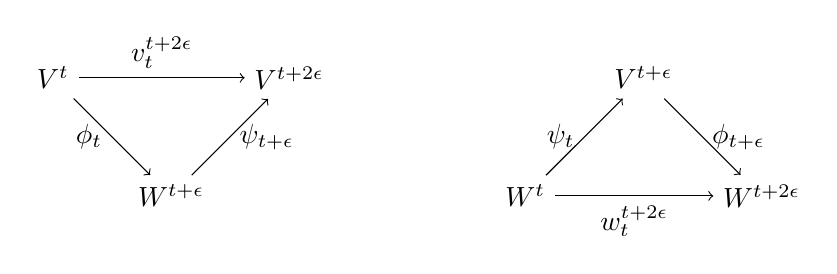
\begin{tikzpicture}
                \node at (0,0) (vt) {$V^t$};
                \node at (3,0) (v2e) {$V^{t+2\epsilon}$};
                \node at (1.5,-1.5) (we) {$W^{t+\epsilon}$};
    
                \node at (7.5,0) (ve) {$V^{t+\epsilon}$};
                \node at (6,-1.5) (wt) {$W^t$};
                \node at (9,-1.5) (w2e) {$W^{t+2\epsilon}$};

                \draw[->] (vt) --node[left]{$\phi_t$} (we);
                \draw[->] (vt) --node[above]{$v_t^{t + 2\epsilon}$} (v2e);
                \draw[->] (we) --node[right]{$\psi_{t + \epsilon}$} (v2e);

                \draw[->] (wt) --node[left]{$\psi_t$} (ve);
                \draw[->] (wt) --node[below]{$w_t^{t + 2\epsilon}$} (w2e);
                \draw[->] (ve) --node[right]{$\phi_{t + \epsilon}$} (w2e);
                
            \end{tikzpicture}            
        \end{center}
    \end{figure} 
\end{definition}

\begin{definition}
    The interleaving distance between two persistence modules $V$ and $W$ is defined as
    $$d_i(V, W) = \inf\{\epsilon \ge 0, V \text{ and } W \text{ are }
    \epsilon-\text{ interleaved}\}.$$
\end{definition}

\subsection{Exercises}

\begin{exercise}
    Let $\mathcal{M}$ be the unit circle of $\R^2$, and $X \subset \R^2$ a
    finite subset. Denote the Hausdorff distance $\epsilon =
    d_H(X,\mathcal{M})$. Suppose that $\epsilon$ is small enough. Let
    $\mathbb{U}$ denote the persistence module of the 1st homology of the Cech
    filtration of $X$. Using the stability theorem, deduce the existence of a
    bar in the barcode, and give a lower bound on its persistence. Compare your result with Exercise 51.
\end{exercise}